%package list
\documentclass{article}
\usepackage[top=3cm, bottom=3cm, outer=3cm, inner=3cm]{geometry}
\usepackage{multicol}
\usepackage{graphicx}
\usepackage{url}
%\usepackage{cite}
\usepackage{hyperref}
\usepackage{array}
%\usepackage{multicol}
\newcolumntype{x}[1]{>{\centering\arraybackslash\hspace{0pt}}p{#1}}
\usepackage{natbib}
\usepackage{pdfpages}
\usepackage{multirow}
\usepackage[normalem]{ulem}
\useunder{\uline}{\ul}{}
\usepackage{svg}
\usepackage{xcolor}
\usepackage{listings}
\lstdefinestyle{ascii-tree}{
    literate={├}{|}1 {─}{--}1 {└}{+}1 
  }
\lstset{basicstyle=\ttfamily,
  showstringspaces=false,
  commentstyle=\color{red},
  keywordstyle=\color{blue}
}
%\usepackage{booktabs}
\usepackage{caption}
\usepackage{subcaption}
\usepackage{float}
\usepackage{array}

\newcolumntype{M}[1]{>{\centering\arraybackslash}m{#1}}
\newcolumntype{N}{@{}m{0pt}@{}}


%%%%%%%%%%%%%%%%%%%%%%%%%%%%%%%%%%%%%%%%%%%%%%%%%%%%%%%%%%%%%%%%%%%%%%%%%%%%
%%%%%%%%%%%%%%%%%%%%%%%%%%%%%%%%%%%%%%%%%%%%%%%%%%%%%%%%%%%%%%%%%%%%%%%%%%%%
\newcommand{\itemEmaila}{eportugalpor@unsa.edu.pe}
\newcommand{\itemEmailb}{hchoquehuancaz@unsa.edu.pe}
\newcommand{\itemEmailc}{jmamanices@unsa.edu.pe}
\newcommand{\itemStudenta}{Eduardo Portugal}
\newcommand{\itemStudentb}{Hernan Choquehuanca}
\newcommand{\itemStudentc}{Jhonatan Mamani}
\newcommand{\itemCourse}{Fundamentos de Programación 2}
\newcommand{\itemCourseCode}{1701213}
\newcommand{\itemSemester}{II}
\newcommand{\itemUniversity}{Universidad Nacional de San Agustín de Arequipa}
\newcommand{\itemFaculty}{Facultad de Ingeniería de Producción y Servicios}
\newcommand{\itemDepartment}{Departamento Académico de Ingeniería de Sistemas e Informática}
\newcommand{\itemSchool}{Escuela Profesional de Ingeniería de Sistemas}
\newcommand{\itemAcademic}{2023 - B}
\newcommand{\itemInput}{Del 25 Setiembre 2023} 
\newcommand{\itemOutput}{Al 4 Octubre 2023}
\newcommand{\itemPracticeNumber}{01}
\newcommand{\itemTheme}{Algoritmos de Ordenamiento y Búsqueda en java}
%%%%%%%%%%%%%%%%%%%%%%%%%%%%%%%%%%%%%%%%%%%%%%%%%%%%%%%%%%%%%%%%%%%%%%%%%%%%
%%%%%%%%%%%%%%%%%%%%%%%%%%%%%%%%%%%%%%%%%%%%%%%%%%%%%%%%%%%%%%%%%%%%%%%%%%%%

\usepackage[english,spanish]{babel}
\usepackage[utf8]{inputenc}
\AtBeginDocument{\selectlanguage{spanish}}
\renewcommand{\figurename}{Figura}
\renewcommand{\refname}{Referencias}
\renewcommand{\tablename}{Tabla} %esto no funciona cuando se usa babel
\AtBeginDocument{%
	\renewcommand\tablename{Tabla}
}

\usepackage{fancyhdr}
\pagestyle{fancy}
\fancyhf{}
\setlength{\headheight}{30pt}
\renewcommand{\headrulewidth}{1pt}
\renewcommand{\footrulewidth}{1pt}
\fancyhead[L]{\raisebox{-0.2\height}{
\includegraphics[width=3cm]{img/logo_episunsa.png}}}
\fancyhead[C]{\fontsize{7}{7}\selectfont	\itemUniversity \\ \itemFaculty \\ \itemDepartment \\ \itemSchool \\ \textbf{\itemCourse}}
\fancyhead[R]{\raisebox{-0.2\height}{
\includegraphics[width=1.2cm]{img/logo_abet}}}
\fancyfoot[L]{Estudiantes: Eduardo, Hernan, Jhonatan}
\fancyfoot[C]{Página \thepage}
\fancyfoot[R]{\itemCourse}

% para el codigo fuente
\usepackage{listings}
\usepackage{color, colortbl}
\definecolor{dkgreen}{rgb}{0,0.6,0}
\definecolor{gray}{rgb}{0.5,0.5,0.5}
\definecolor{mauve}{rgb}{0.58,0,0.82}
\definecolor{codebackground}{rgb}{0.95, 0.95, 0.92}
\definecolor{tablebackground}{rgb}{0.8, 0, 0}

\lstset{frame=tb,
	language=bash,
	aboveskip=3mm,
	belowskip=3mm,
	showstringspaces=false,
	columns=flexible,
	basicstyle={\small\ttfamily},
	numbers=none,
	numberstyle=\tiny\color{gray},
	keywordstyle=\color{blue},
	commentstyle=\color{dkgreen},
	stringstyle=\color{mauve},
	breaklines=true,
	breakatwhitespace=true,
	tabsize=3,
	backgroundcolor= \color{codebackground},
}


%---------------------------------------------------------------------------------------
\begin{document}
	
	\vspace*{10px}
	
	\begin{center}	
		\fontsize{17}{17} \textbf{ Informe de Práctica en Teoría \itemPracticeNumber}
	\end{center}
	\centerline{\textbf{\Large Tema: \itemTheme}}
	%\vspace*{0.5cm}	

	\begin{flushright}
		\begin{tabular}{|M{2.5cm}|N|}
			\hline 
			\rowcolor{tablebackground}
			\color{white} \textbf{Nota}  \\
			\hline 
			     \\[30pt]
			\hline 			
		\end{tabular}
	\end{flushright}	

	\begin{table}[H]
        
		\begin{tabular}{|x{4.7cm}|x{4.8cm}|x{4.8cm}|}
        
			\hline 
			\rowcolor{tablebackground}
			\color{white} \textbf{Estudiantes} & \color{white}\textbf{Escuela}  & \color{white}\textbf{Asignatura}   \\
			\hline 
			{\itemStudenta \par \itemEmaila \par \itemStudentb \par \itemEmailb \par \itemStudentc \par \itemEmailc} & {\par \itemSchool} & {\par \itemCourse \par Semestre: \itemSemester \par Código: \itemCourseCode}     \\
			\hline 			
		\end{tabular}
	\end{table}
	
	\begin{table}[H]
		\begin{tabular}{|x{4.7cm}|x{4.8cm}|x{4.8cm}|}
			\hline 
			\rowcolor{tablebackground}
			\color{white}\textbf{Practica} & \color{white}\textbf{Tema}  & \color{white}\textbf{Duración}   \\
			\hline 
			\itemPracticeNumber & \itemTheme & 5 días   \\
			\hline 
		\end{tabular}
	\end{table}
	
	\begin{table}[H]
		\begin{tabular}{|x{4.7cm}|x{4.8cm}|x{4.8cm}|}
			\hline 
			\rowcolor{tablebackground}
			\color{white}\textbf{Semestre académico} & \color{white}\textbf{Fecha de inicio}  & \color{white}\textbf{Fecha de entrega}   \\
			\hline 
			\itemAcademic & \itemInput &  \itemOutput  \\
			\hline 
		\end{tabular}
	\end{table}
	
	\section{Tarea}
	\begin{itemize}		
		\item Elaborar un proyecto utilizando git. donde se elabore un sistema para ingresar datos de alumnos universitarios. (Clase Student)
            \item El sistema debe almacenar los estudiantes en un Array. (Considerar leer archivos CSV).
            \item Implemente el algoritmo de ordenamiento por Inserción(Iterativo-Cuadrático) para ordenar el arreglo de estudiantes por diferentes parámetros. Ejemplo: Por apellido, paterno.
            \item Descubra cuál es el tiempo que se demora en las ejecuciones.
            \item Explique cualquier otro algoritmo de ordenamiento de complejidad logarítmica. e implemente el ordenamiento utilizando los mismo parámetros anteriores.
            \item Grafique los resultados de las simulaciones realizadas considerando como unidad de medida los nanosegundos. Desde n=1 alumno hasta n=N alumnos.
            \item Luego, para el arreglo ordenado implemente el algoritmo de búsqueda binaria iterativo/recursivo y grafique los resultados de sus simulaciones.

	\end{itemize}
		
	\section{Equipos, materiales y temas utilizados}
	\begin{itemize}
		\item Sistema Operativo Windows 11 Home Single Language 22H2 64 bits.
        \item Sistema Operativo Ubuntu versión 22.04.3 LTS
		\item Visual Studio Code 1.82.2.0.
		\item JDK 17 Full 64-Bits 17.0.7.7.
		\item Git 2.41.0.2.
		\item Cuenta en GitHub con el correo institucional.
        \item Arreglos Estándar y de Objetos.
        \item JFreeChart 1.5.3.
        \item JCommon 1.0.22.
	\end{itemize}
	
	\section{URL de Repositorio Github}
	\begin{itemize}
		\item URL del Repositorio GitHub para clonar o recuperar.
		\item \url{https://github.com/hernanchoquehuanca/fp2-23b.git}
		\item URL para el práctica 01 en el Repositorio GitHub.
		\item \url{https://github.com/hernanchoquehuanca/fp2-23b/tree/main/fase01/prac01}
	\end{itemize}

	\section{Trabajo de Práctica 01}
	
	\begin{itemize}	
		\item A continuación se muestra el desarrollo del trabajo grupal de la práctica 01:
	\end{itemize}

 %%%%%%%%%%%%%%%%%% DESDE AQUI EMPIEZAN LAS PARTES DEL CÓDIGO

    \subsection{Creación de la clase Student y sus atributos}

    %%% ATRIBUTOS
	\begin{itemize}	
		\item Se crea la clase Student, que contendrá atributos de distintos tipos de variables:
        \begin{itemize}
            \item String: email, nombre, apellido materno, apellido paterno.
            \item boolean: género, estado.
            \item int: CUI, fecha de nacimiento.
        \end{itemize}
	\end{itemize}

	\lstinputlisting[language=Java, firstline=1, lastline=4, firstnumber=1, caption={Atributos de la clase "Student"},numbers=left,]{src/Student.java}
 
    %%% MÉTODO CONSTRUCTOR
    \begin{itemize}	
		\item Se agregó el método constructor, este método asigna los distintos datos recibidos sobre el estudiante haciendo uso de los setters, que con según un arreglo llamado data considera para cada índice un atributo.
	\end{itemize}

    \lstinputlisting[language=Java, firstline=6, lastline=15, firstnumber=1, caption={Método constructor de la clase "Student"},numbers=left,]{src/Student.java}

    %%% SETTERS
    \begin{itemize}	
		\item Se implementaron los setters respetivos a cada atributo de la clase, teniendo en consideración el tipo de variable recibida.
        \item En los atributos del tipo String, sea el CUI, fecha de nacimiento, genero y estado se consideró el tipo de variable que se debe asignar.
        \begin{itemize}
            \item cui: se asignaba el substring que contiene a los últimos 8 caracteres.
            \item dateBirth: el entero asignado al atributo se componía de una cadena al que se extraía los valores númericos considerando sus posiciones (año, mes, día).
            \item gender: al recibir tanto 1 (masculino) o 0 (femenino) como valor del género, asignando asi un booleano al atributo donde true representa el género masculino y false al femenino.
            \item status: de manera similar en el estado se consideraba el 1 como activo y el 0 como inactivo, de esta manera se asignaba tanto true como false respectivamente al atributo.
        \end{itemize}
	\end{itemize}

    \lstinputlisting[language=Java, firstline=17, lastline=50, firstnumber=1, caption={Setters de la clase "Student"},numbers=left,]{src/Student.java}

    %%% GETTERS
    
    \begin{itemize}	
		\item Como parte de la clase, también se agregaron los getters correspondientes a cada atributo.
	\end{itemize}

    \lstinputlisting[language=Java, firstline=53, lastline=76, firstnumber=1, caption={Getters de la clase "Student"},numbers=left,]{src/Student.java}


	%%% Bufferedreader y Bufferedwriter

    \subsection{Lectura de archivos csv utilizando Bufferedreader y Bufferedwriter}
	
	\begin{itemize}	
		\item Se crea un BufferedReader llamado Lines para leer el archivo especificado (StudentData).
		\item Utiliza un bucle while para leer cada línea del archivo usando readLine().
        \item Incrementa numLine por cada línea leída, lo que resulta en el conteo total de líneas en el archivo.
	\end{itemize}


	\lstinputlisting[language=Java, firstline=80, lastline=85, firstnumber=80, caption={Clase "Student"},numbers=left,]{src/Student.java}
    
    \lstinputlisting[language=Java, firstline=118, lastline=134, firstnumber=118, caption={Clase "StudentRegistration"},numbers=left,]{src/StudentRegistration.java}

    %%% INTERFAZ 1 PARA RECIBIR LOS ALGORITMOS A UTILIZAR

    \subsection{Interfaz 1 - Recepción de algoritmos de ordenamiento a utilizar}
    
    \begin{itemize}
        \item La primera interfaz tiene como fin interactuar con el usuario de manera que se seleccione el dato a ordenar como también los algoritmos que desee utilizar para luego mostrar la grafica con su comparación.
        \begin{itemize}
            \item Primeramente se asigna tanto el tamaño como nombre de ventana y configurarla para cuando se realice el cierre de ventana.
        \end{itemize}
    \end{itemize}
    \lstinputlisting[language=Java, firstline=34, lastline=36, firstnumber=1, caption={},numbers=left,]{src/StudentRegistration.java}

    \begin{itemize}
        \begin{itemize}
            \item Se crean 3 JPanel, que sirven para la organización tanto de espacios de elementos y botones.
        \end{itemize}
    \end{itemize}
    \lstinputlisting[language=Java, firstline=38, lastline=40, firstnumber=38, caption={},numbers=left,]{src/StudentRegistration.java}

    \begin{itemize}
        \begin{itemize}
            \item Se configura las restricciones del diseño, para ordenarlos de manera que tenga una mejor apariencia.
        \end{itemize}
    \end{itemize}
    \lstinputlisting[language=Java, firstline=42, lastline=43, firstnumber=42, caption={},numbers=left,]{src/StudentRegistration.java}

    \begin{itemize}
        \begin{itemize}
            \item Se crea las etiquetas y un JComboBox que contendrá los algoritmos de ordenamiento, de esta manera el usuario podrá marcar las que desee utilizar.
        \end{itemize}
    \end{itemize}
    \lstinputlisting[language=Java, firstline=45, lastline=47, firstnumber=45, caption={},numbers=left,]{src/StudentRegistration.java}

    \begin{itemize}
        \begin{itemize}
            \item Se crean distintos checkBoxes utilizando el arreglo de algorithm e inicializandolos en false, ya que estos cambiarán si es que el usuario decide seleccionarlos.
            \item Posterior a ello utilizando ActionListener se obtienen las checkbox, que se actualizan en caso sea marcado o desmarcado (varie su valor booleano).
        \end{itemize}
    \end{itemize}
    \lstinputlisting[language=Java, firstline=49, lastline=61, firstnumber=49, caption={},numbers=left,]{src/StudentRegistration.java}

    \begin{itemize}
        \begin{itemize}
            \item Se ubican los componentes que se encontrarán en el panerlSuperior.
        \end{itemize}
    \end{itemize}
    \lstinputlisting[language=Java, firstline=63, lastline=72, firstnumber=63, caption={},numbers=left,]{src/StudentRegistration.java}

    \begin{itemize}
        \begin{itemize}
            \item Creación de un panel que contendrá las JCheckBox y agregandolas al panelSuperior.
        \end{itemize}
    \end{itemize}
    \lstinputlisting[language=Java, firstline=74, lastline=81, firstnumber=74, caption={},numbers=left,]{src/StudentRegistration.java}

    \begin{itemize}
        \begin{itemize}
            \item Se hace un llamado al método sortingAlgorithms utilizando el ActionListener al interactuar con el botón creado.
            \item Además se toma en cuenta las excepciones que se produzcan durante la ejecución del código.
        \end{itemize}
    \end{itemize}
    \lstinputlisting[language=Java, firstline=83, lastline=95, firstnumber=83, caption={},numbers=left,]{src/StudentRegistration.java}

    \begin{itemize}
        \begin{itemize}
            \item Se declara e inicializa el boton2, que servirá para llamar al método con la segunda interfaz (Búsqueda).
        \end{itemize}
    \end{itemize}
    \lstinputlisting[language=Java, firstline=97, lastline=104, firstnumber=97, caption={},numbers=left,]{src/StudentRegistration.java}

    \begin{itemize}
        \begin{itemize}
            \item Finalmente se agregan los botones al panel que los contendrá.
            \item Se estructura la ventana principal colocando los paneles y sus ubicaciones.
            \item Se ubica y muestra la ventana de la interfaz.
        \end{itemize}
    \end{itemize}
    \lstinputlisting[language=Java, firstline=106, lastline=113, firstnumber=106, caption={},numbers=left,]{src/StudentRegistration.java}

    \begin{figure}[H]
        \centering
	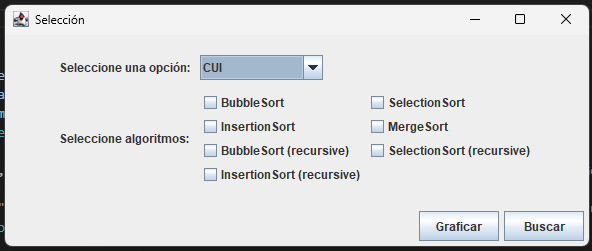
\includegraphics[width=0.8\textwidth,keepaspectratio]{img/Interfaz1.png}
        \caption{Interfaz 1}
    \end{figure}
    
    %%% INTERFAZ 2 PARA REALIZAR LA búsqueda BINARIA 
    
    \subsection{Interfaz 2 - Búsqueda Binaria de datos ordenados}

    \begin{itemize}
        \item Esta segunda interfaz va dirigida a la interacción con el usario para realizar la búsqueda de un estudiante ingresando un dato específico.
        \item Dentro del método se utiliza el dato ingresaro, para luego según sea el tipo de dato recibido mostrarle los datos completos del estudiante en caso exista dentro del registro.
        \item Para realizar esta búsqueda se hace uso del algoritmo de ordenamiento MergeSort por su eficiencia, luego se invoca a los métodos tanto interativo como recursivo de la búsqueda binaria.
        \item Para este método se utilizó parte del código de la interfaz 1.
        \begin{itemize}
            \item Primeramente se asigna tanto el tamaño como nombre de ventana y configurarla para cuando se realice el cierre de ventana.
        \end{itemize}
    \end{itemize}
    \lstinputlisting[language=Java, firstline=544, lastline=546, firstnumber=544, caption={},numbers=left,]{src/StudentRegistration.java}

    \begin{itemize}
        \begin{itemize}
            \item Se crean 3 JPanel, que sirven para la organización tanto de espacios de elementos y botones.
        \end{itemize}
    \end{itemize}
    \lstinputlisting[language=Java, firstline=548, lastline=550, firstnumber=548, caption={},numbers=left,]{src/StudentRegistration.java}

    \begin{itemize}
        \begin{itemize}
            \item Se configura las restricciones del diseño, para ordenarlos de manera que tenga una mejor apariencia.
        \end{itemize}
    \end{itemize}
    \lstinputlisting[language=Java, firstline=552, lastline=553, firstnumber=552, caption={},numbers=left,]{src/StudentRegistration.java}
    
    \begin{itemize}
        \begin{itemize}
            \item Creación de las etiquetas, comboBox para seleccionar el tipo de dato, y el campo para ingresar el texto del dato a buscar.
        \end{itemize}
    \end{itemize}
    \lstinputlisting[language=Java, firstline=555, lastline=559, firstnumber=555, caption={},numbers=left,]{src/StudentRegistration.java}

    \begin{itemize}
        \begin{itemize}
            \item Creación del botón para la búsqueda.
            \item Configuración del ActionListener para el botón creado.
            \begin{itemize}
                \item Primero se realiza el ordenamiento de los datos en el arreglo principal, según el atributo especificado, y se hace un llamado al método mergeSort
                \item Se realiza un llamado, pero ahora a los algoritmos de búsqueda binaria iterativa y recursiva.
                \item Mientras estas búsquedas son ejecutadas, se considera el tiempo y con los distintos tamaños de datos ya fijados, esto en ambos tipos búsqueda.
                \item Finalmente muestra los resultados de la búsqueda si es que el estudiante con los datos recibidos existe, todo esto mediante una ventana emergente que se muestra luego de llamar al método crearVentana.
                \item Por último muestra la gráfica de los tiempos tomados a través del método graphic.
            \end{itemize}
        \end{itemize}
    \end{itemize}
    \lstinputlisting[language=Java, firstline=561, lastline=604, firstnumber=561, caption={},numbers=left,]{src/StudentRegistration.java}

    \begin{itemize}
        \begin{itemize}
            \item Se configura la ubicación y ubicación de los componentes del diseño, todo esto dentro del panelSuperior
        \end{itemize}
    \end{itemize}
    \lstinputlisting[language=Java, firstline=608, lastline=620, firstnumber=608, caption={},numbers=left,]{src/StudentRegistration.java}

    \begin{itemize}
        \begin{itemize}
            \item Finalmente se agregan los botones y otros componentes al panel que los contendrá.
            \item Se estructura la ventana principal colocando los paneles y sus ubicaciones.
            \item Se ubica y muestra la ventana de la interfaz.
        \end{itemize}
    \end{itemize}
    \lstinputlisting[language=Java, firstline=622, lastline=629, firstnumber=622, caption={},numbers=left,]{src/StudentRegistration.java}

     \begin{figure}[H]
        \centering
	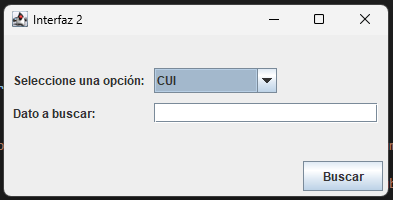
\includegraphics[width=0.8\textwidth,keepaspectratio]{img/Interfaz2.png}
        \caption{Interfaz 2}
    \end{figure}

    %%% MÉTODO CREAR VENTANA

    \begin{itemize}
        \begin{itemize}
            \item Como fue mencionado antes, se utilizó un método llamado , el cual será explicado:
            \begin{itemize}
                \item Se crea la ventana y sus características.
                \item Se agrega un JLabel para mostrar el texto y se agrega a la ventana.
                \item Por último es mostrado, actualizando el texto y usando formato en HTML.
            \end{itemize}
        \end{itemize}
    \end{itemize}
    \lstinputlisting[language=Java, firstline=633, lastline=649, firstnumber=633, caption={},numbers=left,]{src/StudentRegistration.java}

     \begin{figure}[H]
        \centering
	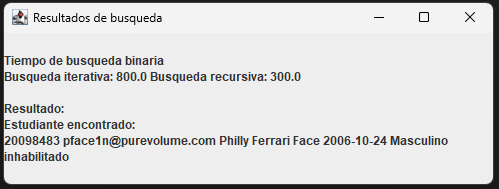
\includegraphics[width=0.8\textwidth,keepaspectratio]{img/Result_Search.png}
        \caption{Ventana con los datos encontrados}
    \end{figure}
 
 %%% ALGORITMOS DE ORDENAMIENTOOOOOOOOOOOOOOOOO

    \subsection{Creación de los algoritmos de ordenamiento}
    
        \begin{itemize}	
            \item Para iniciar con la creación de los algoritmos se tuvo que definir qué datos se iban a comparar (CUI, email, nombres, etc.), para esto, en la selección de algoritmos se define a la variable 'orden' de la siguiente forma:
        \end{itemize}
        
        \lstinputlisting[language=Java, firstline=86, lastline=95, firstnumber=406, caption={Obtención del valor de orden},numbers=left,]{src/StudentRegistration.java}

        \begin{itemize}
            \item El evento (ActionEvent) se desencadena cuando ocurre la acción de hacer click en el botón.
            \item El TRY CATCH de la línea 408, se ejecutará cuando ocurra esto.
            \item Se obtiene el índice del elemento seleccionado en un ComboBox llamado comboBoxDate y se asigna a la variable 'orden'.
            \item Con este dato guardado, se procede a llamar a la ejecución de los algoritmos de ordenamiento.
            \item Finalmente, se capturan posibles excepciones de tipo IOException que puedan ocurrir al llamar al método sortingAlgorithms() y en caso de existir, se imprime un mensaje de error.
        \end{itemize}

        %%%
        
    \subsubsection{Método comparison() para el ordenamiento}

    \lstinputlisting[language=Java, firstline=406, lastline=435, firstnumber=406, caption={Creación del método para comparar en el ordenamiento},numbers=left,]{src/StudentRegistration.java}

        \begin{itemize}	
            \item Este método fue creado para comparar dos objetos de la clase Student basándose en el criterio especificado previamente por el parámetro orden (tipo de dato a comparar).
            \item Como se ve en los casos, se comparan los valores de cada uno de los tipos de datos de los estudiantes.
            \item Se retorna el resultado de la comparación (result), que puede tener un valor menor, mayor o igual a 0. Menor a 0, si el primer objeto resulta de menor valor que el segundo, mayor a 0 en caso contrario y 0 si ambos tienen el mismo valor.
        \end{itemize}

    %%% BUBBLE SORT ITERATIVO
    
    \subsubsection{Algoritmo Bubble Sort}
        
    \lstinputlisting[language=Java, firstline=222, lastline=233, firstnumber=222, caption={Creación del algoritmo Bubble Sort iterativo},numbers=left,]{src/StudentRegistration.java}
     
        \begin{itemize}	
            \item Se toma como único argumento el arreglo de objetos Student (arr) que se va a ordenar.
            \item Con el bucle FOR exterior de la línea 223, se itera sobre el arreglo desde el segundo elemento (i = 1) hasta el último elemento (i = arr.length - 1).
            \item El bucle FOR interior de la línea 224, itera sobre el arreglo desde el primer elemento hasta el penúltimo elemento. Será el encargado de recorrer los elementos para intercambiar si se cumple la condición de IF.
            \item La condicional IF en la línea 225, compara dos elementos adyacentes en el arreglo utilizando la función comparison(), el de la posición actual del bucle interior y el que le sigue, de ser mayor el primero, deberán intercambiarse.
        \end{itemize}

    %%% BUBBLE SORT RECURSIVO
    
    \subsubsection{Algoritmo Bubble Sort recursivo}
    
    \lstinputlisting[language=Java, firstline=236, lastline=253, firstnumber=236, caption={Creación del algoritmo Bubble Sort recursivo},numbers=left,]{src/StudentRegistration.java}
     
        \begin{itemize}	
            \item En este método recursivo se recibe el arreglo arr y la longitud del mismo.
            \item El primer caso condicional del IF en la líne 237 presenta el caso base de la recursión. Ya que, cuando n es igual a 1, la recursión se detiene y el arreglo se considera ordenado.
            \item Se inicializa un contador 'count' para mantener un seguimiento de los intercambios realizados en cada iteración.
            \item El bucle FOR de la línea 242 compara cada elemento con su siguiente en el arreglo y realiza un intercambio como en el caso del iterativo utilizando el método comparison() en el IF de la línea 243.
            \item En la línea 250, el IF indica que si no se realizó ningún intercambio en la iteración actual, el arreglo ya está ordenado y se cierra el método recursivo.
            \item Si existe intercambios, se llama recursivamente al mismo método con n reducido en 1 para los elementos restantes.
        \end{itemize}

	%%% SELECTION SORT ITERATIVO
        \subsubsection{Algoritmo Selection Sort}
        
        \lstinputlisting[language=Java, firstline=256, lastline=267, firstnumber=256, caption={Creación del algoritmo Selection Sort iterativo},numbers=left,]{src/StudentRegistration.java}
        
        \begin{itemize}	
            \item Se recibe únicamente el arreglo de objetos Student (arr) que se va a ordenar.
            \item En la primera linea dentro del método, se obtiene la longitud del arreglo arr y se almacena en la variable n.
            \item En primer lugar, se inicializa como el índice del elemento más pequeño al valor de i.
            \item Este elemento se evalúa con el bucle FOR en la línea 256 y el IF integrado  para buscar en la parte del arreglo que aún no se ha ordenado, el elemento con el menor valor. 
            \item Tras haber encontrado el elemento más pequeño en el índice "min-idx", se intercambia con el primer elemento aún no ordenado del arreglo que va reduciendose hasta haber comparado todo.  
        \end{itemize}

        %%% SELECTION SORT RECURSIVO
        \subsubsection{Algoritmo Selection Sort recursivo}

        \begin{itemize}	
            \item Se crea un método de apoyo llamado "minIndex":
        \end{itemize}
        
        \lstinputlisting[language=Java, firstline=282, lastline=292, firstnumber=282, caption={Método de apoyo minIndex},numbers=left,]{src/StudentRegistration.java}
     
        \begin{itemize}	
            \item Este método ayudará a encontrar el índice del elemento mínimo en un rango dado (i a j) del arreglo arr ingresado de forma recursiva.
            \item La condición IF de la línea 283, devuelve el índice i si es igual al valor del índice j.

        \end{itemize}

        \lstinputlisting[language=Java, firstline=270, lastline=281, firstnumber=270, caption={Creación del algoritmo Selection Sort recursivo},numbers=left,]{src/StudentRegistration.java}

        \begin{itemize}
            \item En el método de ordenación principal, se toma como argumentos el arreglo arr, su longitud, y el índice idx para controlar la posición actual durante el proceso de selección.
            \item La primera condición en el IF de la línea 271, evalúa si el index del elemento es igual al tamaño del arreglo para finalizar su ejecución. 
            \item En la línea 274, el valor de k, llama a la función minIndex() para encontrar el índice del elemento mínimo desde la posición idx hasta el final del arreglo (n - 1).Al finalizar esa recursión, k es el índice del elemento mínimo encontrado.
            \item Al igual que el iterativo, compara los elementos del mínimo y la posición inicial de la parte desordenada para intercambiarlos si no son iguales haciendo la comparación con el método comparison().
            \item Finalmente, el proceso recursivo continúa, mientras se excluye el elemento más pequeño que ya está en su posición correcta modificando el index como: idx + 1.
        \end{itemize}

	%%% INSERTION SORT ITERATIVO
        \subsubsection{Algoritmo Insertion Sort}

        \lstinputlisting[language=Java, firstline=295, lastline=307, firstnumber=295, caption={Creación del algoritmo Insertion Sort iterativo},numbers=left,]{src/StudentRegistration.java}
        
        \begin{itemize}	
            \item El único argumento recibido es el arreglo de los objetos que se va a ordenar.
            \item En las líneas siguientes, se declara una variable j para representar una posición en el arreglo y una variable key para almacenar temporalmente un elemento durante el proceso de ordenamiento.
            \item Se declara el elemento en la posición i del arreglo como la clave para comparar 
            \item El bucle WHILE de la línea 301, compara el elemento clave con los elementos anteriores a él (posición j) para encontrar su posición adecuada. Mientras arr[j] es mayor que el elemento la clave, se desplaza y se reduce el valor de j para continuar la comparación hacia atrás.
            \item Finalmente, la clave se inserta en la posición correcta (j + 1) y se continúa con el ciclo.  
        \end{itemize}

        %%% INSERTION SORT RECURSIVO
        \subsubsection{Algoritmo Insertion Sort recursivo}

        \lstinputlisting[language=Java, firstline=310, lastline=323, firstnumber=310, caption={Creación del algoritmo Insertion Sort recursivo},numbers=left,]{src/StudentRegistration.java}

        \begin{itemize}	
            \item En este método se toma como argumentos el arreglo de objetos Student arr y su longitud n.
            \item Se crea una condición con un IF en la línea 311 para acabar el método si queda un elemento o si no hay ninguno, ya que se consideraría ya ordenado.
            \item El método recursivo ordena los primeros n-1 elementos. 
            \item Se toma como clave (key) al último elemento del arreglo, posteriormente, inicializamos j con n - 2 para asegurar que apunte al último elemento de la parte ordenada. 
            \item El bucle WHILE de la línea 318, compara el elemento clave con los elementos anteriores a él (en posición j) para encontrar su posición adecuada.
            \item Finalmente, una vez encuentra su ubicación, se inserta en la posición correcta de su orden.
        \end{itemize}

 	%%% MERGE SORT
        \subsubsection{Algoritmo Merge Sort}

        \begin{itemize}
            \item Se crea un primer método "merge" que recibe el arreglo de objetos Student (arr), los índices de los extremos izquierdo (l) y derecho (r) de un subarreglo y un índice intermedio (m).

        \end{itemize}
        
        \lstinputlisting[language=Java, firstline=335, lastline=370, firstnumber=335, caption={Creación del método Merge},numbers=left,]{src/StudentRegistration.java}
        
        \begin{itemize}	
            \item Se inicializa n1 y n2. n1 representará la cantidad de elementos en el primer subarreglo (L) y n2 representará la cantidad de elementos en el segundo subarreglo (R). 
            \item Posteriormente, divide el arreglo en dos subarreglos ordenados (L y R) en base a la posición intermedia m. Combina los subarreglos ordenados L y R en el arreglo principal arr.
        \end{itemize}

        \lstinputlisting[language=Java, firstline=326, lastline=333, firstnumber=326, caption={Creación del método Merge Sort},numbers=left,]{src/StudentRegistration.java}

        \begin{itemize}
            \item Toma tres parámetros: el arreglo de objetos Student (arr), y los índices de los extremos izquierdo (l) y derecho (r) del subarreglo que debe ordenarse. \item Divide recursivamente el arreglo en subarreglos más pequeños hasta que los subarreglos contengan un solo elemento. Entre las líneas 329 y 331 llama a la función merge para combinar y ordenar los subarreglos.
	\end{itemize}

	%%%

    \subsection{Creación de los algoritmos de búsqueda}

        %%% MÉTODO COMPARISON SEARCH
    \subsubsection{Método comparisonSearch para la búsqueda binaria}
    
    \lstinputlisting[language=Java, firstline=438, lastline=476, firstnumber=438, caption={Creación de método para comparar en la búsqueda},numbers=left,]{src/StudentRegistration.java}
        
        \begin{itemize}	
            \item Este método realiza comparaciones entre un objeto Student y un dato de tipo String que se modificará según los criterios específicos (CUI, email, nombre, apellidos, fecha de nacimiento, género y estado) establecidos en un SWITCH CASE que se basa en el orden definido.
            \item El criterio básico, es la devolución de un valor positivo cuando el primer valor es mayor, uno negativo si es menor, y devuelve 0 si los dos son iguales.
	\end{itemize}
 
    %%%
    
    \subsubsection{Algoritmo de Búsqueda Binaria Iterativa}

    \lstinputlisting[language=Java, firstline=375, lastline=387, firstnumber=375, caption={Creación de algoritmo Búsqueda Binaria Iterativa},numbers=left,]{src/StudentRegistration.java}
        
        \begin{itemize}	
            \item El método recibe el arreglo ordenado de objetos y el String x que se buscará.
            \item El entero 'l',  recibe el índice izquierdo inicial del arreglo (0). Y el entero 'r' toma el valor del índice derecho inicial del arreglo (tamaño del arreglo menos 1).
            \item El bucle while de la línea 377 se ejecuta mientras el índice izquierdo (l) sea menor o igual al índice derecho (r), lo que permite saber si aún hay elementos en el rango de búsqueda.
            \item Dentro del ciclo WHILE, el valor de 'm' se calcula como el índice medio del rango actual (entre l y r). Esto nos asegura que se compara el objeto medio.
            \item Con el IF de la línea 379, se compara el objeto en la posición m del arreglo con el valor buscado x utilizando el método comparisonSearch(). Si la comparación resulta en 0, se ha encontrado el valor y se devuelve el índice m del objeto hallado.
            \item En cambio, en el IF de la línea 381, cuando la comparación es menor que 0, se infiere que el valor buscado está en la mitad derecha del rango actual, se actualiza el valor de l = m + 1.
            \item En el ELSE en la línea 383, queda la comparación mayor a 0, lo cual, indica que el valor buscado está en la mitad izquierda del rango actual, y se actualiza r según corresponda
            \item Por útlimo, si no se encuentra el valor después de completar el bucle, se devuelve -1 para indicar que el valor no se ha encontrado en el arreglo.
	\end{itemize}

    %%%
 
    \subsubsection{Algoritmo de Búsqueda Binaria Recursiva}

    \lstinputlisting[language=Java, firstline=390, lastline=401, firstnumber=390, caption={Creación de algoritmo Búsqueda Binaria Recursiva},numbers=left,]{src/StudentRegistration.java}
        
        \begin{itemize}	
            \item Se toma como argumentos el arreglo ordenado arr, los índices l y r que representan los límites izquierdo y derecho de la búsqueda, y un String x que es el elemento que se busca.
            \item La condional IF de la línea 391 verifica si el límite derecho r es mayor o igual que el límite izquierdo l. Si esto es verdadero, se continúa con la búsqueda, en caso contrario, ya se ha recorrido el arreglo y no se encontró x (devuelve -1).
            \item Se calcula el índice medio del rango actual de búsqueda.
            \item En el primer IF de la línea 393 se realiza una comparación con el método comparisonSearch() entre el objeto de la posición media y el valor que se busca, al igual que en el iterativo, si son iguales se devuelve inmediatamente el índice m.
            \item En el siguiente IF, en la línea 395, si la comparación resulta mayor a 0, se sigue la búsqueda recursiva en la mitad izquierda.
            \item Por último, si no se cumple ninguno (comparación menor a 0), en la línea 398, la búsqueda recursiva se continúa en la mitad derecha del arreglo.
	\end{itemize}
 
 
	%%%

    \subsection{Gráfica lineal de los algoritmos de ordenamiento/búsqueda}
    
    \subsubsection{Varibles para el registro de tiempos}
    
    \lstinputlisting[language=Java, firstline=20, lastline=22, firstnumber=20, caption={Variables Globales para el tiempo},numbers=left,]{src/StudentRegistration.java}
	
	\begin{itemize}	
		\item Para el registro de los tiempos de ejecución de los datos, en la línea 20 se declararon 2 variable globales de tipos long para registrar el tiempo en nanosegundos, antes y después de ejecutar los algoritmos de ordenamiento y búsqueda.
        \item De igual forma en la línea 21 se declararon dos arreglos bidimensionales (timesSaved) (timeDataAB) de doubles donde se registrarán todos los registros de tiempo de los 7 algoritmos de ordenamiento y de los 2 algoritmos de búsqueda respectivamente.
        \item Finalmente, en la línea 22 se declararon dos variables de tipo double donde se registrará el último tiempo registrado de los algoritmos de búsqueda, que luego se mostrarán en pantalla.
	\end{itemize}

    \subsubsection{Registro de tiempos de ejecución en los algoritmos de ordenamiento}

    \lstinputlisting[language=Java, firstline=136, lastline=214, firstnumber=136, caption={Registro de los tiempos de ejecución - algoritmos de ordenamiento},numbers=left,]{src/StudentRegistration.java}
	
	\begin{itemize}	
        \item En un comienzo se colocaron las variables de tiempo dentro de cada algoritmo lo cual registraba el tiempo que se demoraba el algoritmo en ordenar cada elemento, sin embargo esto no permitía obtener los gráficos que necesitábamos.
        \item Luego se optó por colocar las variables antes y después de llamar al método del algoritmo de ordenamiento, para poder registrar el tiempo que demora en el ordenamiento de todos los elementos.
        \item El buble FOR de la línea 137 permite realizar la obtención de los datos de tiempo, teniendo en cuenta una variación en la cantidad de elementos a ordenar, que va aumentando sucesivamente.
		\item En la línea 143 se puede apreciar que se declara e inicializa un arreglo al cual se le copian los elementos originales del arreglo principal, y esto se realiza con todos los métodos, logrando que cada uno de los algoritmos de ordenamiento reciba un arreglo que pueda ordenar.
        \item En la línea 214 se hace un llamado al método graphic(1) con el parámetro 1 para que realice la gráfica lineal de los tiempos de los algoritmos de ordenamiento.
	\end{itemize}

    \subsubsection{Registro de tiempos de ejecución en los algoritmos de búsqueda}
    
    \lstinputlisting[language=Java, firstline=565, lastline=604, firstnumber=565, caption={Registro de los tiempos de ejecución - algoritmos de ordenamiento},numbers=left,]{src/StudentRegistration.java}
	
	\begin{itemize}	
		\item Para ejecutar los algoritmos de búsqueda primero se debe ordenar el arreglo, por lo que se llama al método mergeSort para ordenar los elementos dependiendo de lo que el usuario quiera buscar.
        \item Si el usuario quiere buscar un nombre, entonces el ordenamiento será según los nombres.
        \item En la línea 576 se puede apreciar que se declara e inicializa un arreglo al cual se le copian los elementos originales del arreglo principal, y esto también se realiza antes del otro método, logrando que cada uno de los algoritmos de búsqueda reciba un arreglo en donde buscar.
        \item En la línea 578 y 580 se registran los tiempos antes y después de realizada la búsqueda binaria iterativa, lo mismo sucede con la recursiva, y luego la resta de ambos valores se guarda en sus respectivas variables.
        \item El bucle FOR de la línea 575 permite realizar la obtención de los datos de tiempo, teniendo en cuenta una variación en la cantidad de elementos donde se va a realizar la búsqueda, que va aumentando sucesivamente.
        \item En la línea 594 existe una condicional que determina que si con el dato especificado se logró encontrar al estudiante o no. Si el valor a evaluar es -1 entonces no se encontró al estudiante, si cualquier otro número, este representara el índice y por lo tanto la ubicación del elemento dentro del arreglo.
        \item En la línea 604 se hace un llamado al método graphic(2) con el parámetro 2 para que realice la gráfica lineal de los tiempos de los algoritmos de ordenamiento.
	\end{itemize}

    \subsubsection{Gráficas lineales}
    \lstinputlisting[language=Java, firstline=481, lastline=537, firstnumber=481, caption={Método para crear la gráfica lineal},numbers=left,]{src/StudentRegistration.java}

    \begin{itemize}
        \item El método recibe un entero que permitirá diferenciar si la gráfica es para los algoritmos de ordenamiento o para los de búsqueda.
        \item En la condicional de la línea 485 en caso de que el número sea 1, se hará referencia a la gráfica de los algoritmos de ordenamiento, se crearan las series de aquellos algoritmos que hayan sido seleccionados en la primera interfaz (línea 491) y también se añadirán sus registros de tiempos a las series (línea 493).
        \item En caso de que el número sea diferente de 1, se hará referencia a la gráfica de los algoritmos de búsqueda, se crearan las series de los dos algoritmos (línea 501 y 502) y también se añadirán sus registros de tiempos a las series (línea 505)
        \item En la línea 508 se crea el objeto llamado "dataset" del tipo XYSeriesCollecion, luego, en las siguientes líneas se agregan todas las series al conjunto de datos "dataset".
        \item Se crea la variable chart que será el grafico que representara los datos, seguidamente se especifican el título de la gráfica, los títulos del ejeX y del ejeY, el conjunto de datos, la orientación del gráfico, y otros parámetros booleanos (mostrar leyendas, mostrar etiqueta de herramienta emergente, generar una URL para el gráfico).
        \item Luego de las líneas 520 a la 532, se establecen otros parámetros y características de la gráfica, para que, finalmente la sentencia de la línea 532 permita la visualización de la gráfica.
	\end{itemize}

    \subsection{Commits}

    \begin{lstlisting}[language=bash,caption={Comit n°1}][H]		
		$ git add .
		$ git commit -m "Creamos la clase Student.java con los atributos necesarios, además del archivo StudentRegistration.java. Por el  momento lee los archivos .csv y los imprime (utilizando arreglos estándar)"
      $ git push -u origin main
	\end{lstlisting}

    \begin{itemize}
        \item En este commit de registro la creación de la clase Student.java con todos sus atributos, métodos mutadores, métodos accesores y el método toString para que se impriman los objetos con todos sus datos.
    \end{itemize}
    
    \begin{lstlisting}[language=bash,caption={Comit n°2}][H]		
		$ git add .
		$ git commit -m "Creando arreglos de datos del tiempo, crendo un metodo grafic que permite realizar una grafica lineal de los datos"
      $ git push -u origin main
	\end{lstlisting}

    \begin{itemize}
        \item Commit realizado para añadir los arreglos creados que se encargarán de registrar los tiempos de ejecución de los algoritmos utilizados, asimismo se implementó el método graphic() que crea el gráfico lineal de los tiempos de ejecución. 
    \end{itemize}

    \begin{lstlisting}[language=bash,caption={Comit n°3}][H]		
		$ git add .
		$ git commit -m "Agregando la busqueda binaria recursiva, ademas del metodo comparisionSearch que sera utilizado en la busqueda"
      $ git push -u origin main
	\end{lstlisting}

    \begin{itemize}
        \item Este commit fue realizado para añadir el método que ejecuta la búsqueda binaria recursiva, para su correcto funcionamiento, se creó en conjunto a un método llamado comparisionSearch, que permitió comparar los datos según el parámetro requerido con un SwitchCase implementado.
    \end{itemize}

     \begin{lstlisting}[language=bash,caption={Comit n°4}][H]		
		$ git add .
		$ git commit -m "Implementando los metodos de la interfaz restantes, aunque aun seguiran en revision por posibles errores u omisiones"
      $ git push -u origin main
	\end{lstlisting}

    \begin{itemize}
            \item En el commit se agregó los métodos en la interfaces para interactuar con el usuario, tanto para el ordenamiento, como para la búsqueda.
            \item Pero están en revisión debido a posibles errores en casos específicos.
    \end{itemize}

    \begin{lstlisting}[language=bash,caption={Comit n°5}][H]
      $ git add .
		$ git commit -m "Arreglando útlimos errores de la Búsqueda, versión final"
      $ git push -u origin main
	\end{lstlisting}

    \begin{itemize}
        \item Commit realizado para añadir los últimos cambios en el código para corregir un error dentro de la búsqueda de datos que solo permitía buscar una única vez, con esta corrección ahora se pueden realizar varias búsquedas una después de otra.
    \end{itemize}

 
    \subsection{Compilación y ejecución del programa}

    \begin{lstlisting}[language=bash,caption={Compilacion y ejecución}][H]		
		$ javac -cp jfreechart-1.0.19.jar:jcommon-1.0.23.jar StudentRegistration.java Student.java
        $ java -cp .:jfreechart-1.0.19.jar:jcommon-1.0.23.jar StudentRegistration
	\end{lstlisting}

    \subsubsection{Primera interfaz}
    
     \begin{figure}[H]
        \centering
	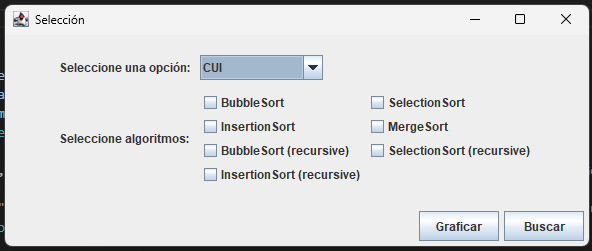
\includegraphics[width=0.8\textwidth,keepaspectratio]{img/Interfaz1.png}
        \caption{Interfaz 1}
    \end{figure}
    
    \begin{itemize}	
        \item El programa le permite al usuario poder seleccionar el atributo con el cual realizará el ordenamiento, además de especificar los algoritmos que desea utilizar, los cuales se mostrarán en la gráfica lineal.
		\item Al hacer click en el botón "Graficar" se mostrará en pantalla el gráfico lineal correspondiente.
		\item Al hacer click en el botón "Buscar" se cerrará automáticamente esta interfaz y se mostrará la segunda interfaz de búsqueda.
	\end{itemize}

    \subsubsection{Gráfico lineal de algoritmos de ordenamiento}
    
     \begin{figure}[H]
        \centering
	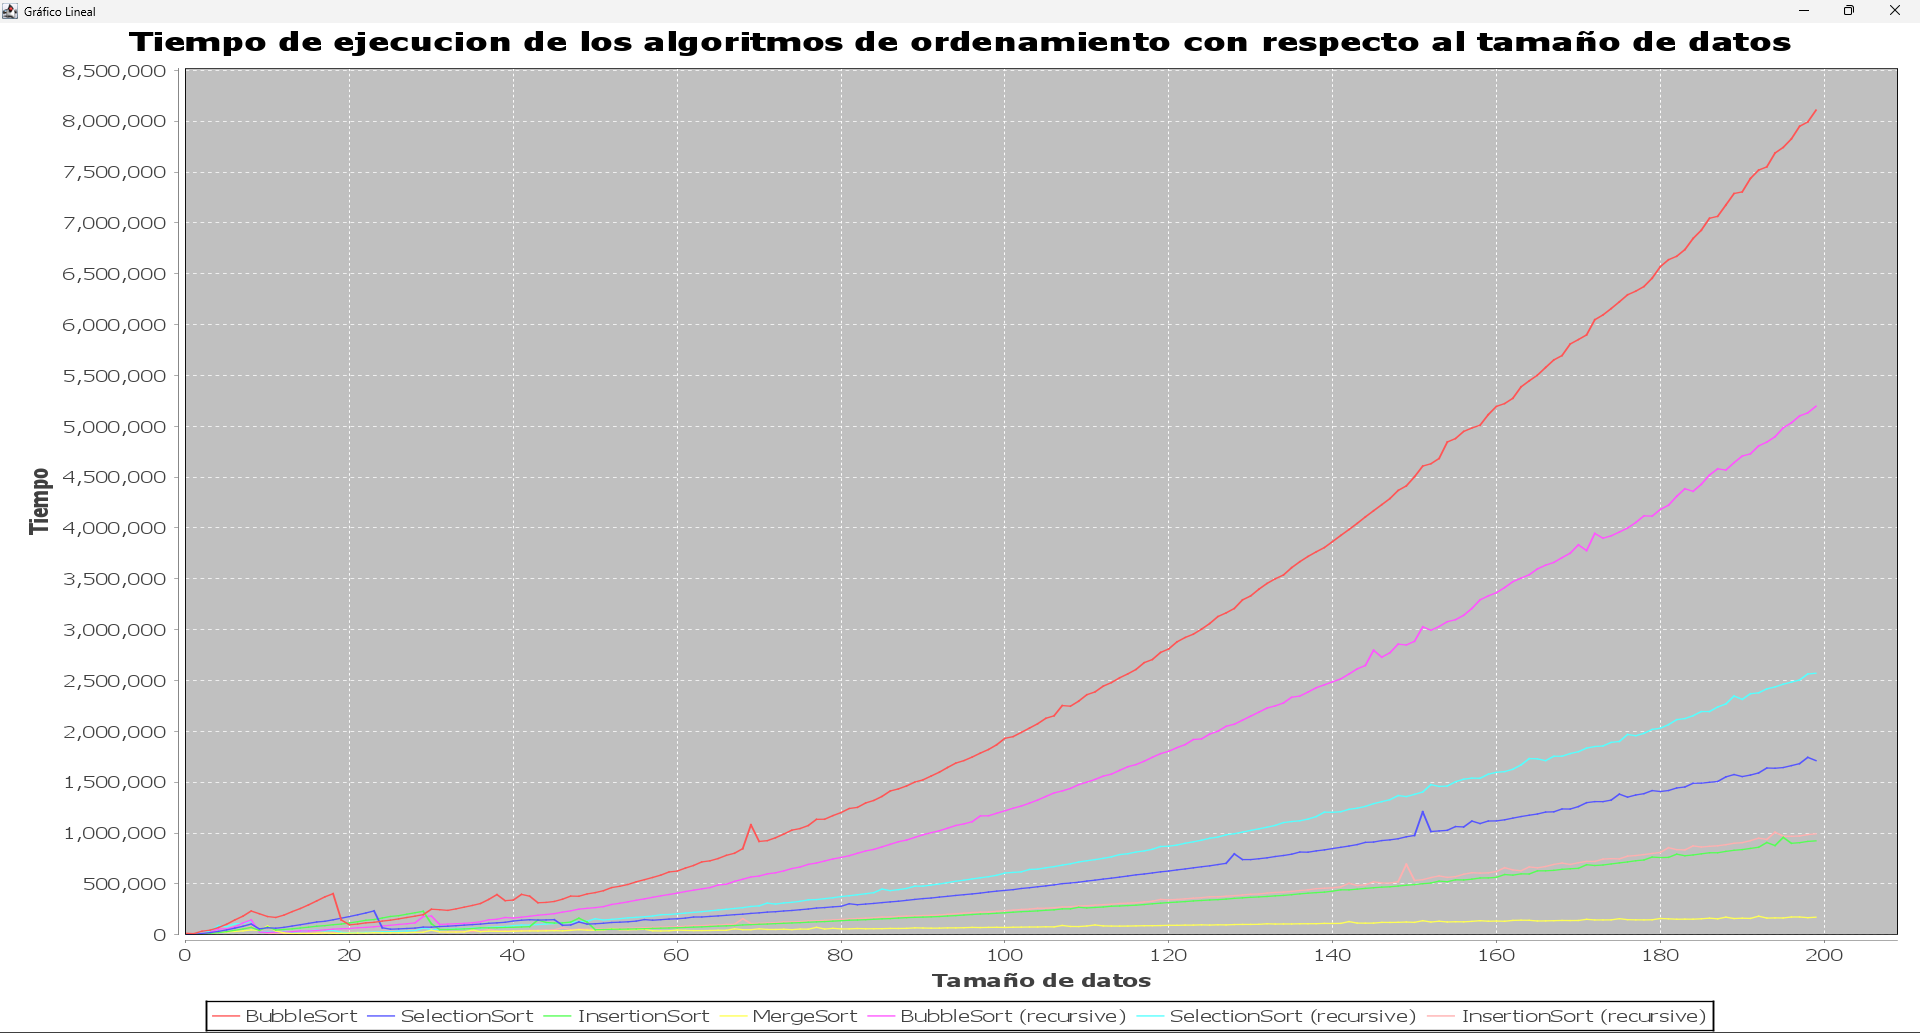
\includegraphics[width=0.8\textwidth,keepaspectratio]{img/Sort_Grafic.png}
        \caption{Gráfico lineal de algoritmos de ordenamiento}
    \end{figure}
    
    \begin{itemize}	
        \item Comparando todos lo gráficos lineales de los tiempos que les toma a los algoritmos ordenar la diferente cantidad de elementos, podemos notar que el algoritmo MergeSort es el más veloz y eficiente para realizar dicho ordenamiento.
        \item Es por esto que, para antes de la ejecución de los algoritmos de búsqueda se optó por usar el algortimo MergeSort por su eficacia. 
	\end{itemize}
    
    \subsubsection{Segunda interfaz}

     \begin{figure}[H]
        \centering
	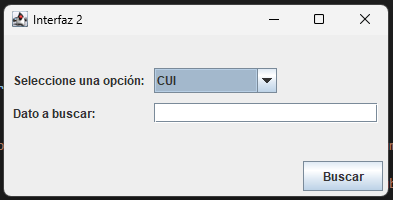
\includegraphics[width=0.7\textwidth,keepaspectratio]{img/Interfaz2.png}
        \caption{Interfaz 2}
    \end{figure}
    
    \begin{itemize}	
        \item Luego de hacer click en el botón "Buscar", automáticamente se abre esta interfaz, la cual le permite al usuario elegir el atributo e ingresar el dato a buscar.
        \item Al hacer click en el botón "" seguidamente se muestra una nueva ventana especificando si el resgistro del estudiante fue encontrado o si no existe, en caso de ser mostrado se imprimirán los datos del estudiante.
        \item Por otro lado, también se mostrará en pantalla el gráfico lineal de los dos algoritmos de ordenamiento.
	\end{itemize}

    \subsubsection{Gráfico lineal de algoritmos de búsqueda}

     \begin{figure}[H]
        \centering
	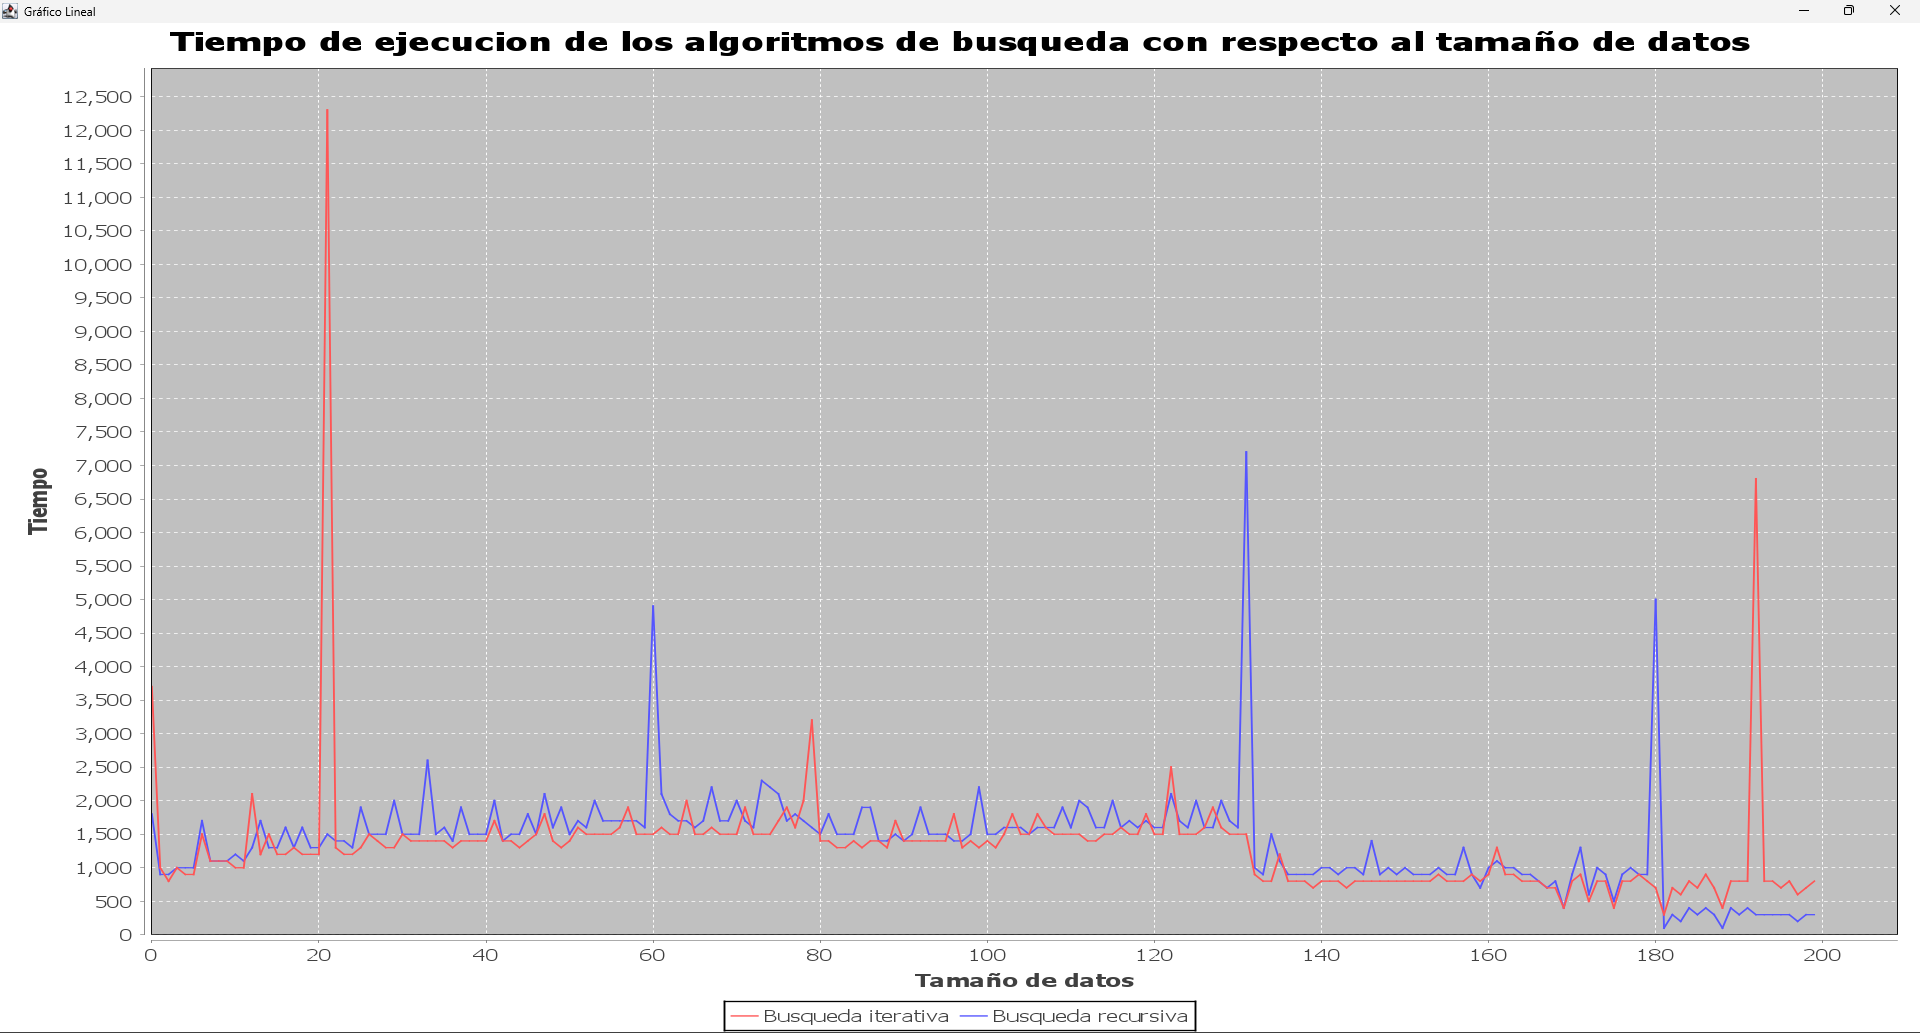
\includegraphics[width=0.8\textwidth,keepaspectratio]{img/Search_Grafic.png}
        \caption{Gráfico lineal de algoritmos de búsqueda}
    \end{figure}
 
	\begin{itemize}	
        \item En la gráfica se puede apreciar los tiempos que le toma a cada algoritmo de búsqueda encontrar el dato ingresado por el usuario, teniendo en cuenta la variación del tamaño de datos entre los cuales se realizará la búsqueda.
		\item Realizando un análisis podemos concluir que el algoritmo de búsqueda binaria (recursiva) resulta ser el mas eficiente y rápido.
	\end{itemize}

    \subsubsection{Ventana de resultado de búsqueda}
 
     \begin{figure}[H]
        \centering
	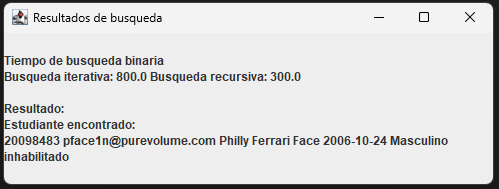
\includegraphics[width=0.8\textwidth,keepaspectratio]{img/Result_Search.png}
        \caption{Ventana de resultado de búsqueda}
    \end{figure}

    \begin{itemize}	
        \item Luego de haberse realizado la búsqueda, en la última ventana son mostrados los resultados de esta.
        \item En caso se encuentre al estudiante en el registro, se mostrarán todos sus datos, como se muestra el la figura 8, caso contrario se le informará al usuario que el dato ingresado no corresponde a ningún estudiante.
	\end{itemize}
	%%%



 %%%%%%%%%%%%%%%%%%

 
	\subsection{Estructura de práctica 01}
	\begin{itemize}	
		\item El contenido que se entrega en este laboratorio es el siguiente:
	\end{itemize}
	
\begin{lstlisting}[style=ascii-tree]
prac01/
|--- jcommon-1.0.23.jar
|--- jfreechart-1.0.19.jar
|--- Student.java
|--- StudentRegistration.java
|--- StudentData.csv
|--- latex
    |--- img
    |   |--- Interfaz1.png
    |   |--- Interfaz2.png
    |   |--- logo_abet.png
    |   |--- logo_episunsa.png
    |   |--- logo_unsa.jpg
    |   |--- Result_Search.png
    |   |--- Search_Grafic.png
    |   |--- Sort_Search.png
    |--- prac01_informe.pdf    
    |--- prac01_informe.tex
    |--- src
        |--- StudentRegistration.java
        |--- Student.java
\end{lstlisting}    

	\section{\textcolor{red}{Rúbricas}}
	
	\subsection{\textcolor{red}{Entregable Informe}}
	\begin{table}[H]
		\caption{Tipo de Informe}
		\setlength{\tabcolsep}{0.5em} % for the horizontal padding
		{\renewcommand{\arraystretch}{1.5}% for the vertical padding
		\begin{tabular}{|p{3cm}|p{12cm}|}
			\hline
			\multicolumn{2}{|c|}{\textbf{\textcolor{red}{Informe}}}  \\
			\hline 
			\textbf{\textcolor{red}{Latex}} & \textcolor{blue}{El informe está en formato PDF desde Latex,  con un formato limpio (buena presentación) y fácil de leer.}   \\ 
			\hline 
			
			
		\end{tabular}
	}
	\end{table}
	
	\clearpage
	
	\subsection{\textcolor{red}{Rúbrica para el contenido del Informe y demostración}}
	\begin{itemize}			
		\item El alumno debe marcar o dejar en blanco en celdas de la columna \textbf{Checklist} si cumplió con el ítem correspondiente.
		\item Si un alumno supera la fecha de entrega,  su calificación será sobre la nota mínima aprobada, siempre y cuando cumpla con todos lo items.
		\item El alumno debe autocalificarse en la columna \textbf{Estudiante} de acuerdo a la siguiente tabla:
	
		\begin{table}[ht]
			\caption{Niveles de desempeño}
			\begin{center}
			\begin{tabular}{ccccc}
    			\hline
    			 & \multicolumn{4}{c}{Nivel}\\
    			\cline{1-5}
    			\textbf{Puntos} & Insatisfactorio 25\%& En Proceso 50\% & Satisfactorio 75\% & Sobresaliente 100\%\\
    			\textbf{2.0}&0.5&1.0&1.5&2.0\\
    			\textbf{4.0}&1.0&2.0&3.0&4.0\\
    		\hline
			\end{tabular}
		\end{center}
	\end{table}	
	
	\end{itemize}
	
	\begin{table}[H]
		\caption{Rúbrica para contenido del Informe y demostración}
		\setlength{\tabcolsep}{0.5em} % for the horizontal padding
		{\renewcommand{\arraystretch}{1.5}% for the vertical padding
		%\begin{center}
		\begin{tabular}{|p{2.7cm}|p{7cm}|x{1.3cm}|p{1.2cm}|p{1.5cm}|p{1.1cm}|}
			\hline
    		\multicolumn{2}{|c|}{Contenido y demostración} & Puntos & Checklist & Estudiante & Profesor\\
			\hline
			\textbf{1. GitHub} & Hay enlace URL activo del directorio para el  laboratorio hacia su repositorio GitHub con código fuente terminado y fácil de revisar. &2 &X &2 & \\ 
			\hline
			\textbf{2. Commits} &  Hay capturas de pantalla de los commits más importantes con sus explicaciones detalladas. (El profesor puede preguntar para refrendar calificación). &4 &X &3 & \\ 
			\hline 
			\textbf{3. Código fuente} &  Hay porciones de código fuente importantes con numeración y explicaciones detalladas de sus funciones. &2 &X &2 & \\ 
			\hline 
			\textbf{4. Ejecución} & Se incluyen ejecuciones/pruebas del código fuente  explicadas gradualmente. &2 &X &2 & \\ 
			\hline			
			\textbf{5. Pregunta} & Se responde con completitud a la pregunta formulada en la tarea.  (El profesor puede preguntar para refrendar calificación).  &2 &X &2 & \\ 
			\hline	
			\textbf{6. Fechas} & Las fechas de modificación del código fuente estan dentro de los plazos de fecha de entrega establecidos. &2 &X &2 & \\ 
			\hline 
			\textbf{7. Ortografía} & El documento no muestra errores ortográficos. &2 &X &2 & \\ 
			\hline 
			\textbf{8. Madurez} & El Informe muestra de manera general una evolución de la madurez del código fuente,  explicaciones puntuales pero precisas y un acabado impecable.   (El profesor puede preguntar para refrendar calificación).  &4 &X &3 & \\ 
			\hline
			\multicolumn{2}{|c|}{\textbf{Total}} &20 & &18 & \\ 
			\hline
		\end{tabular}
		%\end{center}
		%\label{tab:multicol}
		}
	\end{table}
	
\clearpage

\section{Referencias}
	
\begin{itemize}			
	\item \url{https://parzibyte.me/blog/2020/08/30/java-ordenamiento-seleccion/}
	\item \url{http://puntocomnoesunlenguaje.blogspot.com/2015/02/ordenamiento-insercion-directa-java.html}
        \item \url{https://www.geeksforgeeks.org/bubble-sort/}
        \item \url{https://www.geeksforgeeks.org/insertion-sort/}
        \item \url{https://www.geeksforgeeks.org/selection-sort/}
        \item \url{https://www.geeksforgeeks.org/java-program-for-merge-sort/}
        \item \url{https://www.geeksforgeeks.org/binary-search/}
        \item \url{https://docs.oracle.com/javase/8/docs/api/java/lang/Object.html}
        \item \url{https://docs.oracle.com/javase/8/docs/api/java/util/Arrays.html}
        \item \url{https://docs.oracle.com/javase/tutorial/java/javaOO/lambdaexpressions.html}
        \item \url{https://docs.oracle.com/javase/8/docs/api/java/lang/Exception.html}
        \item \url{https://www.jfree.org/jfreechart/}
        \item \url{https://docs.oracle.com/javase%2F7%2Fdocs%2Fapi%2F%2F/javax/swing/package-summary.html}
\end{itemize}
	%%% 
%\clearpage
%\bibliographystyle{apalike}
%\bibliographystyle{IEEEtranN}
%\bibliography{bibliography}
			
\end{document}